\section{Theorie}
\label{sec:Theorie}

Wird in einen Ionenkristall, der aus einfach geladenen Ionen besteht, ein zweifach geladenes Kation eingebaut, so entsteht an einem Gitterplatz, der normalerweise von einem einfach geladenen Kation besetzt wäre eine Leerstelle.
Zwischen dieser und dem zweiwertigen Kation bildet sich ein Dipolmoment $\vec{p}$ aus, dessen Richtung zunächst willkürlich verteilt ist. Da sich beide Enden auf Gitterplätzen befinden müssen, sind nur diskrete Änderung der Dipolrichtung möglich. Bei Temperaturen $T<\SI{500}{\kelvin}$ können sich nur die Leerstellen auf den Gitterplätzen bewegen, wenn sie die nötige Aktivierungsenergie $W$ besitzen. Nach der Stefan-Boltzmann-Verteilung kann, mit der Boltzmannkonstante $k_.B$, ein Anteil von $\mathrm{e}^{\frac{W}{k_.BT}}$ der Leerstellen bereits durch thermische Bewegung den Gitterplatz wechseln.
Die mittlere Zeit zwischen zwei Dipolrichtungsänderung wird Relaxationszeit genannt und ist gegeben durch
\begin{equation}
\tau=\tau_.0\mathrm{e}^{-\frac{W}{k_.BT}}\label{eq:tau}
\end{equation}
mit der charakteristischen Relaxationszeit $\tau_.0$.
Wird an den Kristall ein elektrisches Feld $E$ angeschlossen, richten sich, gestört durch die bereits vorhandene thermische Energie, ein Teil $y$ der Dipole entlang der Feldrichtung aus. Er lässt sich beschreiben als
\begin{equation}
y=\coth(\frac{p E}{k_.B T})-\frac{k_.BT}{pE}\label{eq:y1},
\end{equation}
mit dem Betrag des Dipolmoments $p$ und der Boltzmann-Konstante $k_.B$. 
Für hohe Temperaturen, also wenn gilt
\[
pE\ll k_.BT,
\]
kann Formel \eqref{eq:y1} näherungsweise beschrieben werden als
\begin{equation}
y=\frac{pE}{3k_.BT}\text{.}\label{eq:y}
\end{equation}
Durch schnelles Abkühlen auf eine Temperatur $T_.0$ steigt nach \eqref{eq:tau} die Relaxationszeit stark an, sodass $y=y(T_.p)$ mit der Polarisationstemperatur $T_.p$ als konstant angenommen werden kann.
Durch Erhitzen mit einer konstanten Heizrate $b$ steigt die thermische Energie, sodass die Dipole wieder eine statistische Richtungsverteilung annehmen. Der resultierende Depolarisationsstrom $i(T)$ folgt Abbildung \ref{fig:i}, jedoch wird er in der Realität bei höheren Temperaturen von einem weiteren Maximum überlagert.
Es gilt mit der Rate der pro Volumen- und Zeiteinheit relaxierenden Dipole $\frac{\mathrm{d}N}{\mathrm{d}t}$ und dem Probenquerschnitt $F$ für den Strom
\begin{equation}
i(T)=F y(T_.p)p\frac{\mathrm{d}N}{\mathrm{d}t}\text{.}\label{eq:i1}
\end{equation}
Da der Prozess thermisch aktiviert ist, ist die Änderung der ausgerichteten antiproportional zur Zahl der noch vorhandenen orientierten Dipole und lässt sich somit über die DGL
\[
\frac{\mathrm{d}N}{\mathrm{d}t}=-\frac{N}{\tau(T)}
\]
beschreiben.
Das Lösen dieser DGL liefert mit der Zahl der zu Beginn bei $T=T_.0$ orientierten Dipole $N_.p$
\begin{equation}
N=N_.p\mathrm{e}^{-\frac{1}{b}\int_{T_.0}^T\frac{\mathrm{d}T'}{\tau(T')}}\text{.}\label{eq:N}
\end{equation}
Mit den Gleichungen \eqref{eq:tau}, \eqref{eq:y} und \eqref{eq:i1} ergibt sich so
\begin{equation}
i(T)=F\frac{p^2E}{3k_.BT_.p}\frac{N_.p}{\tau_.0}\mathrm{e}^{-\frac{1}{b\tau_.0}\int_{T_.0}^T\mathrm{e}^{-\frac{W}{k_.BT'}}\mathrm{d}T'}\cdot \mathrm{e}^{-\frac{W}{k_.BT}}\text{.}\label{eq:i2}
\end{equation}
Für kleine Temperaturen verschwindet das Integral im Exponent, sodass sich $i$ im Anfangsbereich der Stromkurve nähern lässt zu
\begin{equation}
i_.{kl}(T)\approx F\frac{p^2E}{3k_.BT_.p}\frac{N_.p}{\tau_.0}\mathrm{e}^{-\frac{W}{k_.BT}}\text{.}\label{eq:i_kl}
\end{equation}
Logarithmieren liefert 
\begin{equation}
\ln\left(\frac{i}{i_.0}\right)=-\frac{W}{k_.B}\cdot\frac{1}{T}+const\text{.}\label{eq:ln1}
\end{equation}
Für den gesamten Kurvenverlauf lässt sich die Polarisation $P$ des Kristalls betrachten, die ebenfalls der DGL
\begin{equation}
\frac{\mathrm{d}P}{\mathrm{d}t}=-\frac{P}{\tau(T)}\label{eq:DGL}
\end{equation}
folgt und deren Änderung den Strom
\[
i(t)=F\frac{\mathrm{d}P}{\mathrm{d}t}
\]
bewirkt. Da sich für $t\rightarrow\infty$ alle Dipolrichtungen wieder statistisch verteilt haben und somit gilt $P(\infty)=0$, liefert eine Integration
\[
\int_{t(T)}^{\infty}i(t')\mathrm{d}t'=-F P(t)\text{.}
\]
Eingesetzt in \eqref{eq:DGL}, unter Berücksichtigung, dass $T$ eine lineare Funktion von $t$ mit Steigung $b$ ist, mit einer hinreichend großen Temperatur $T^*$, bei der $i$ bereits auf $i\approx\SI{0}{\pico\ampere}$ abgefallen ist und mit Gleichung \eqref{eq:tau}
\begin{equation}
\mathrm{e}^{\frac{W}{k_.BT}}=\frac{\int_{T}^{T^*}i(T')\mathrm{d}T'}{b\tau_.0 i(T)}=\frac{I(T)}{b\tau_.0 i(T)}\text{.}\label{eq:i3}
\end{equation}
Logarithmieren liefert
\begin{equation}
\ln\left(\frac{I(T)}{i(T)\cdot const}\right)=\frac{W}{k_.B}\cdot\frac{1}{T}\text{.}\label{eq:ln2}
\end{equation}
Trägt man die linke Seite der Gleichungen \eqref{eq:ln1} und \eqref{eq:ln2} gegen $\frac{1}{T}$ auf, lässt sich $W$ aus der Steigung der entstehenden Gerade bestimmen.
Wenn die Ableitung der Gleichung \eqref{eq:i2} nach der Temperatur $=0$ ist, ist bei $T=T_.{max}$ das Maximum des Polarisationsstroms.
Das liefert eine Beziehung zur Berechnung von $\tau_.0$:
\begin{equation}
\tau_.0=\frac{k_.BT^2_.{max}}{W b}\mathrm{e}^{-\frac{W}{k_.BT_.{max}}}\text{.}\label{eq:tau0}
\end{equation}
\begin{figure}
	\centering
	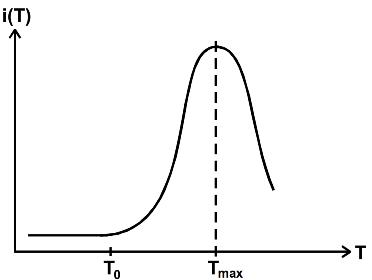
\includegraphics[width=\linewidth-70pt,height=\textheight-70pt,keepaspectratio]{content/images/Verlauf.jpg}
	\caption{Verlauf des Deploarisationsstroms $i(T)$ \cite{V48}.}
	\label{fig:i}
\end{figure}